\section{Project Management}
\subsection{Planning}

The applicative projet only last a semester, but the sigma race is only the $3^{rd}$ of June, so we didn't planned to accomplish all the work only during the \textbf{AP}.\footnote{Short for applicative project} Instead, we decide to focus first on what was the original goal of our AP, driving autonomously in a simulator.\\

As we opted for this AP kind of late\footnote{We first heard of it mid October, we had to think about it, and then we had to do all the proceeding for our inscription.}, we really started working on it arround beginning of November. The first thing to do was to documented ourselves about Machines Learning, Deep Learning, existing software on the domain\dots\\
We gave ourselves a month to gather information about the state of the art in machine learning in autonomous car, but it's such a big domain that we only scratched the surface.


\begin{figure}[!h]
\centering
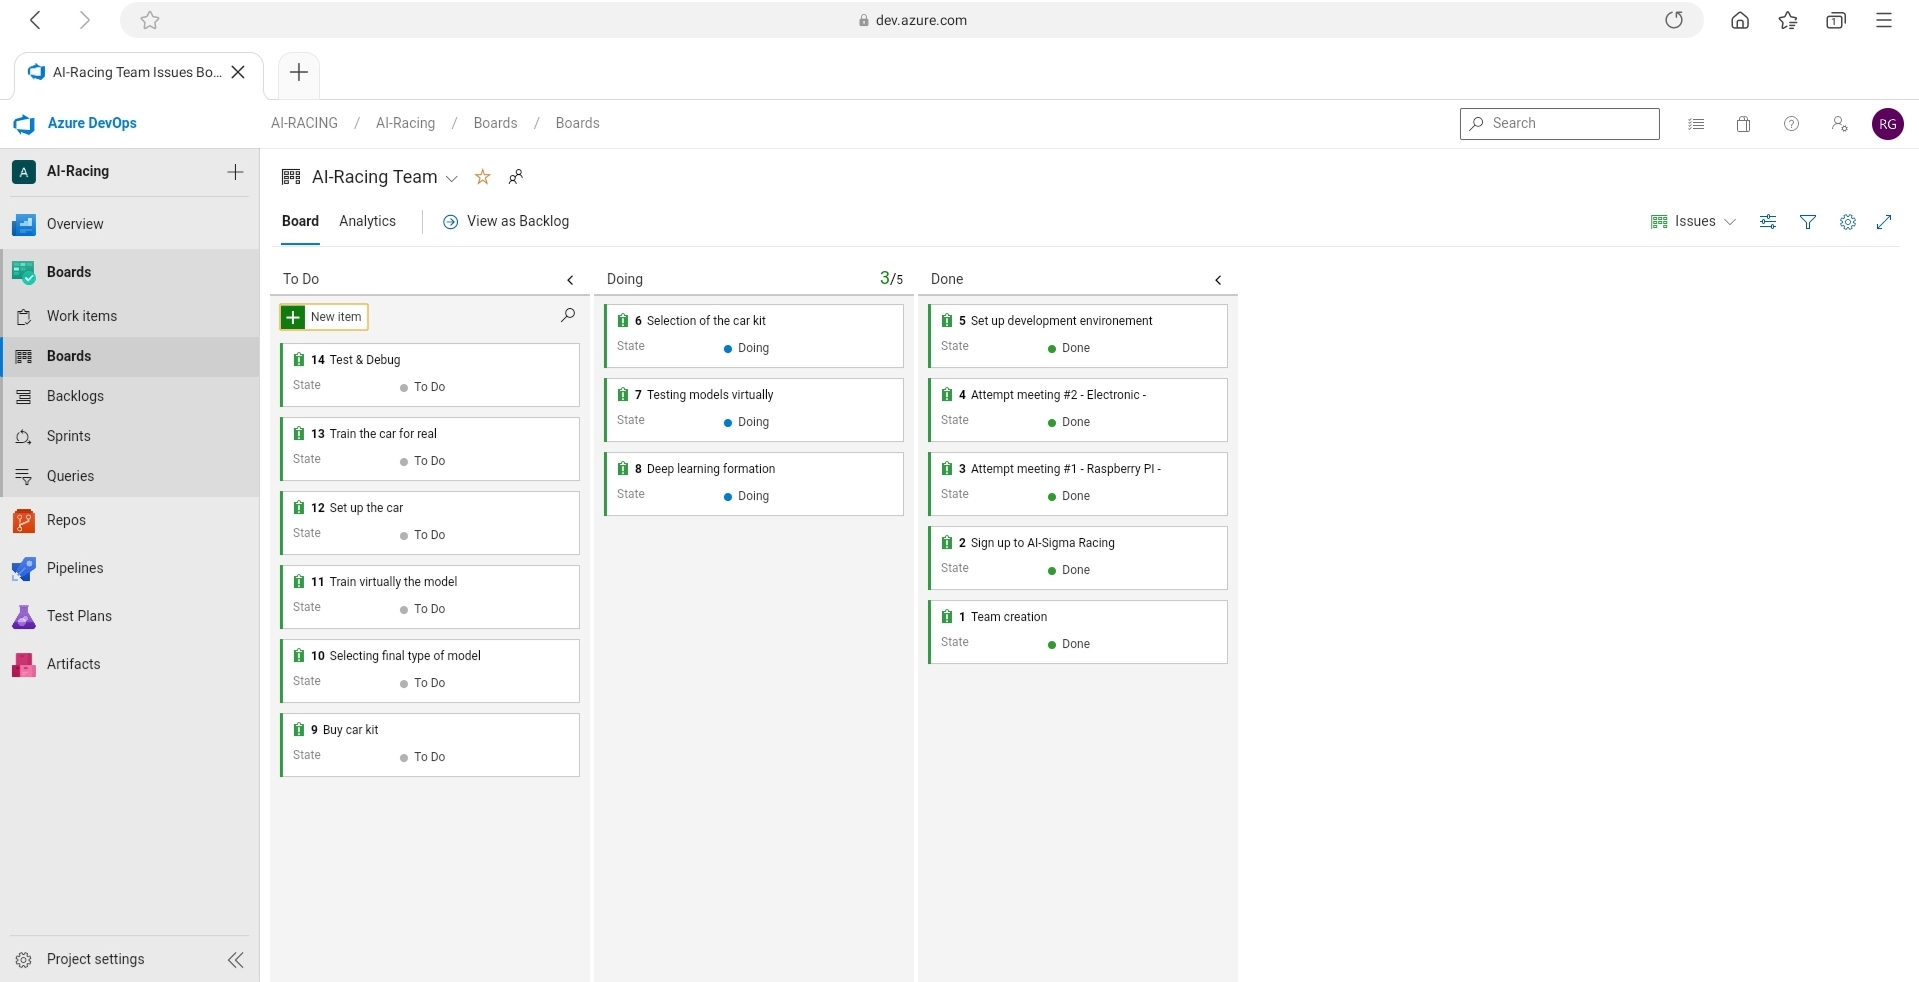
\includegraphics[scale=0.24]{img/devops.jpg}
\caption{We decided to use \textbf{Azure DevOps} to manage our project}
\end{figure}



\subsection{Meetings}
\begin{wrapfigure}{r}{0.4\textwidth}
\centering
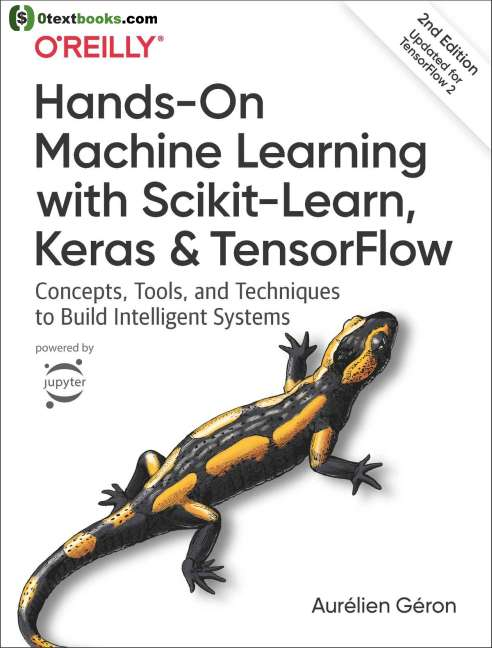
\includegraphics[height=5cm]{img/handsonml.jpeg}
\caption{The book Cyprien bought}
\end{wrapfigure}
As we are flatmates, it was pretty easy to do meetings, we used to do a meeting every week or so, in order to share the result of our research. We both start reading book about Machine Learning and Deep Learning in order to understand how this kind of AI are working\cite{2ndEd}.

\clearpage



\begin{figure}[!h]
\centering
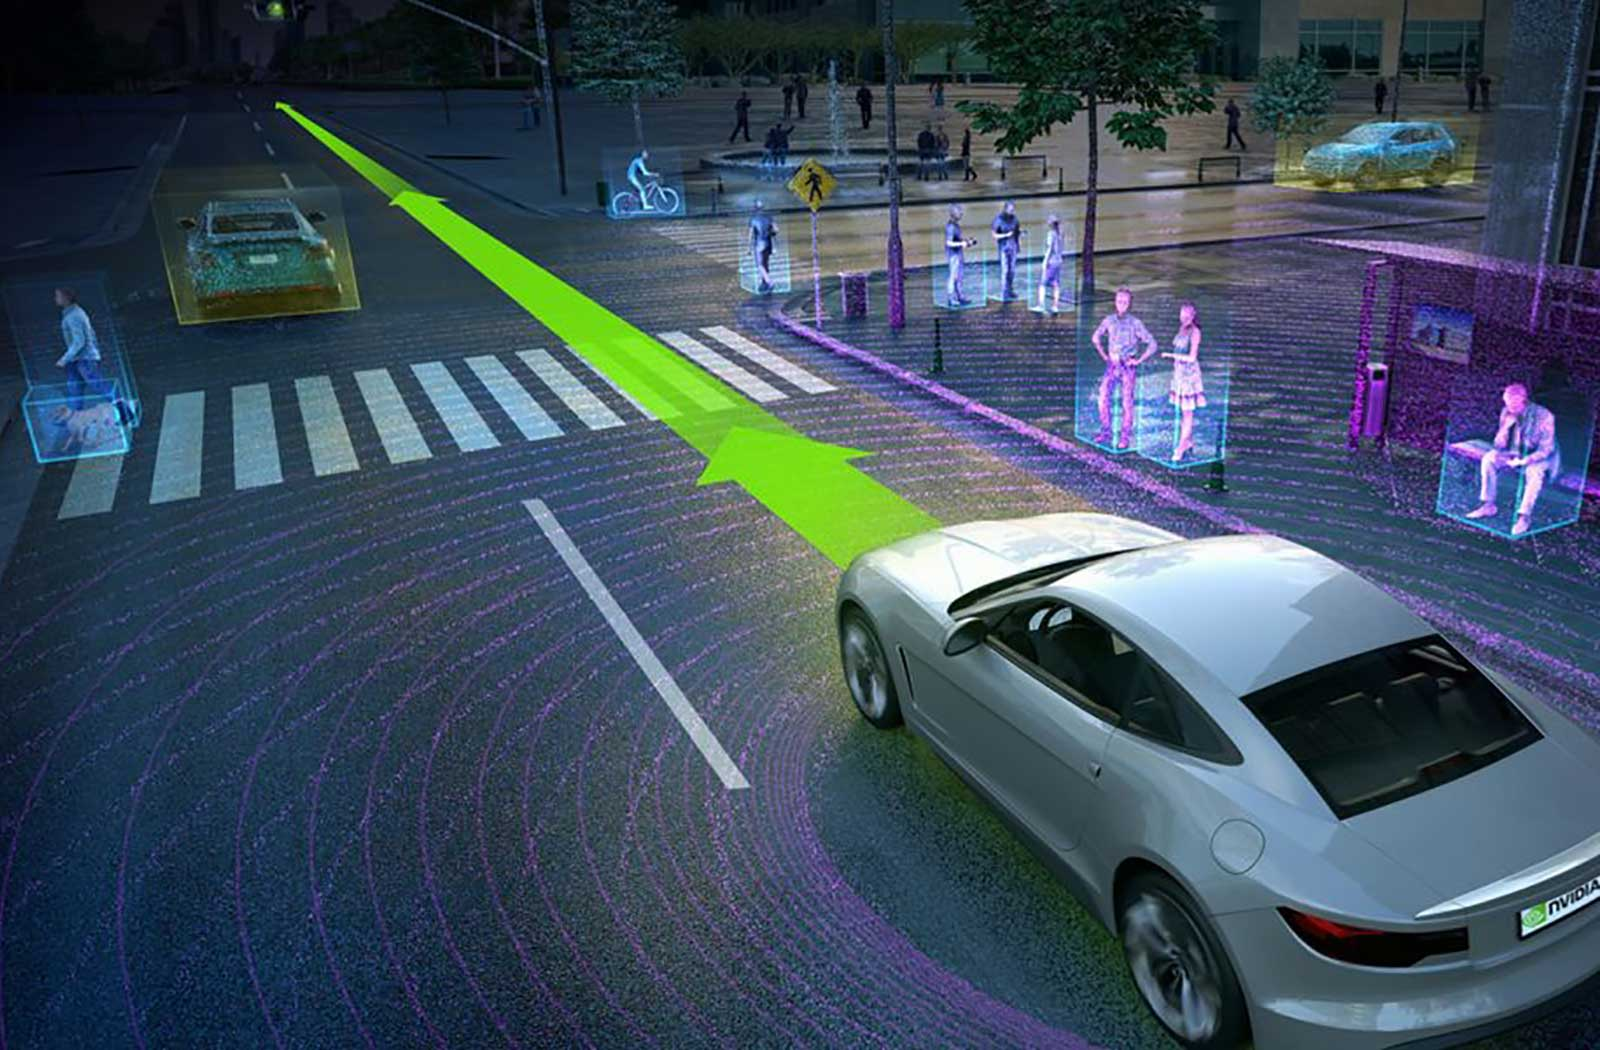
\includegraphics[width=10cm]{img/autonomous_driving.jpeg}
\end{figure}

\subsection{Division of labor}

We divided the work as follow:
\begin{itemize}
\item Cyprien had to setup the simulator
\item Romain had to design a lane detection algorithm 
\item We had to do research on our own to compare deep-learning models to find the best for our situation.
\end{itemize}
\clearpage
